\documentclass[leqno]{article}
\usepackage[utf8]{inputenc}
\usepackage{enumitem}
\usepackage{tikz}
\usepackage[parfill]{parskip}
\usepackage{mathtools}
\usepackage{amsmath}
\usepackage{amssymb}

\title{Computationele logica}
\author{
    Kamans, Jim\\
    \texttt{10302905}
    \and
    Roosingh, Sander\\
    \texttt{11983957}
    \and
    Schenk, Stefan\\
    \texttt{11881798}
}
\date{December 2017}

\begin{document}

\maketitle

\textbf{Possibility:} $\sim_a \coloneqq \leq_a \cup \geq_a$

\textbf{Information Cell:} $w(a) \coloneqq \{s\in W:w\sim_a s\}$

\textbf{Knowledge:} $\lVert K_a \varphi \rVert_M = \{s\in W:s(a) \subseteq
\lVert \varphi \rVert_M\}$

\textbf{Conditional Belief:} $\lVert B_a^\varphi \psi \rVert_M = \{s \in
W:best_a(\lVert\varphi\rVert_M \cap s(a)) \subseteq \lVert\psi\rVert_M\}$


%%%%%%%%%%%%%%%%%%%%%%%%%%%%%%%%%%%%%%%%%%%%%%%%%%%%%%%%%%%%%%%%%%%%%%%%%%%%%%%
%% Exercise 1 %%
%%%%%%%%%%%%%%%%%%%%%%%%%%%%%%%%%%%%%%%%%%%%%%%%%%%%%%%%%%%%%%%%%%%%%%%%%%%%%%%
\section*{Exercise 1}
For this exercise, please use the semantic definitions (given in the slides of
Lectures 4.1 and 4.2) of knowledge $K\varphi$ in plausibility models, belief
$B\varphi$, conditional belief $B^\varphi \psi$ and safe belief $\square
\varphi$ (defined as the Kripke modality for the plausibility relation).

\begin{enumerate}[label=(\alph*)]
	\item \textit{Show the following equivalence:}
		$$K_a \varphi \Leftrightarrow B_a^{\neg \varphi} false$$
		\textit{Proof.} Let \textbf{S} = $(S, \le_a, \sim_a, ||\cdot||)$ be an 
		arbitrary plausibility model and $s \in S$ also be arbitrary.\\
		To prove our equivalence, we need to prove two implications:
		
		\textbf{Proof of left-to-right direction 
		($K_a \varphi \Rightarrow B_a^{\neg \varphi} false$)}
		
		We assume that $s \models K_a \varphi$. By the semantic definition of $K_a$,
		this means that $s(a) \subseteq ||\varphi||$ (1). By definition of $best_a$, 
		$best_a(||\neg \varphi|| \cap s(a)) \subseteq 
		(||\neg \varphi|| \cap s(a))$. From (1), it follows that 
		$(||\neg \varphi|| \cap s(a)) = \emptyset \subseteq ||false||$. By the 
		semantic definition of conditional belief, this means that 
		$s \models B_a^{\neg \varphi} false$.
		
		\textbf{Proof of right-to-left direction 
		($B_a^{\neg \varphi} false \Rightarrow K_a \varphi$)}
		
		We assume that $s \models B_a^{\neg \varphi} false$. By the semantic 
		definition of conditional belief, this means that 
		$best_a(||\neg \varphi|| \cap s(a)) \subseteq (||\neg \varphi|| \cap s(a)) 
		\subseteq ||false||$. $(||\neg \varphi|| \cap s(a)) \subseteq ||false||$ iff 
		$s(a) \subseteq ||\varphi||$. By the semantic definition of $K_a$, this means
		 that $s \models K_a \varphi$. 
		\hfill $\square$

	\item \textit{Prove semantically the equivalence claimed on Slide 24 of
		Lecture Notes 4.2:}
		$$B_a \varphi \Leftrightarrow \Diamond_a \square_a \varphi$$
		where $\Diamond_a \varphi \coloneqq \neg \square_a \neg \varphi$ is the dual
		modality to safe belief $\square_a$.

		[ANSWER HERE]

	\item \textit{Prove (via a counterexample) that \textbf{safe belief does NOT
		imply strong belief}; i.e. that}
		$$\square_a \varphi \not\Rightarrow Sb_a \varphi$$

        Safe belief in some world $s$ means that $t \models \varphi$ for all $t$ such that 
        $s \leq_a t$.\\
        Strong belief implies that for all worlds reachable from that world, 
        the $\varphi$-worlds are strictly more plausible than the 
        non-$\varphi$-worlds.
        
        In the model below, the real world is denoted by *. In this world 
        $\square_a \varphi$ holds (there are no $a$-arrows pointing towards 
        worlds in which $\varphi$ is not true), but $Sb_a \varphi$ doesn't hold,
         because not all non-$\varphi$-worlds reachable from the real world are
          strictly more plausible than the $\varphi$-worlds reachable from the 
         real world (the middle world is more plausible than the left world).

		\begin{center}
		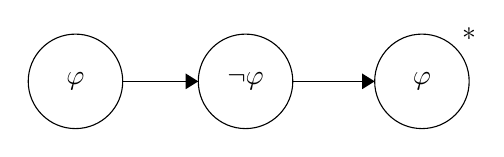
\begin{tikzpicture}[scale=0.2]
		\tikzstyle{every node}+=[inner sep=0pt]
		\draw [black] (7.55,-6.55) circle (3);
		\draw (7.55,-6.55) node {$\varphi$};
		\draw [black] (18.35,-6.55) circle (3);
		\draw (18.35,-6.55) node {$\neg \varphi$};
		\draw [black] (29.55,-6.55) circle (3);
		\draw (29.55,-6.55) node {$\varphi$};
		\draw (32.55,-3.55) node {$*$};
		\draw [black] (10.55,-6.55) -- (15.35,-6.55);
		\fill [black] (15.35,-6.55) -- (14.55,-6.05) -- (14.55,-7.05);
		\draw [black] (21.35,-6.55) -- (26.55,-6.55);
		\fill [black] (26.55,-6.55) -- (25.75,-6.05) -- (25.75,-7.05);
		\end{tikzpicture}
		\end{center}
		\end{enumerate}

\textbf{HINT}: The positive statements (a) and (b) need general proofs: you
need to show that, for \textit{every} plausibility model and \textit{every
sentence} $\phi$, the desired formula is true at \textit{all} the worlds of
that model. But the negative statement (c) must be shown by giving a
counterexample: construct \textit{some} plausibility model and find
\textit{some} sentence $\varphi$ for which the implication fails to be true
at \textit{some} world of that model (which we can think of as the ``real
world'').

%%%%%%%%%%%%%%%%%%%%%%%%%%%%%%%%%%%%%%%%%%%%%%%%%%%%%%%%%%%%%%%%%%%%%%%%%%%%%%%
%% Exercise 2 %%
%%%%%%%%%%%%%%%%%%%%%%%%%%%%%%%%%%%%%%%%%%%%%%%%%%%%%%%%%%%%%%%%%%%%%%%%%%%%%%%
\section*{Exercise 2}

A virtual agent in a video game doesn't know his current position in the
virtual space, but all he cares is (a) whether or not he's in a ``Dangerous''
zone (say, close to a dangerous monster), and (b) whether or not he's close to
this Target (say, a treasure). Let's use the letter $d$ to denote the sentence
\textit{the agent is in a dangerous zone}, and the letter $t$ to denote the
sentence \textit{the agent is close to the target}. These possibilities are
independent of each other, and the agent \textbf{doesn't know} which is the
case, so he \textbf{cannot exclude any} of the four possible cases $d \land t$,
 $d \land \neg t$, $\neg d \land t$ and $\neg d \land \neg t$. However, our
agent \textbf{believes both} that he's close to the target AND that he's NOT in
 a dangerous zone. \textbf{If} he would learn that this belief is WRONG (i.e.
that at least one of his two beliefs is false), then he'd still believe (
conditional on this new information) that he is close to the target. But
\textbf{if} he would learn instead that he's far from (=NOT close to) the
target, then (conditional on this information) he'd keep his initial belief
that he's NOT in a dangerous zone.

\begin{enumerate}
    \item \textit{Write down a logical formula in the language of beliefs,
    knowledge and conditional beliefs to encode all the above assumptions.}

    $\neg K(t) \land \neg K(\neg t) \land \neg K(d) \land \neg K(\neg d) \land
    B(t \land \neg d) \land B^{\neg (t \land \neg d)}(t) \land
    B^{\neg t}(\neg d)$

    \item \textit{Represent the agent's beliefs (and conditional beliefs),
    using a \textbf{plausibility model} with four possible worlds. Specify the
    \textbf{valuation} (which atomic sentences of the two atomic sentences $d$
    and $t$ are true at which worlds). Represent the agent's
    \textbf{plausibility relation} on these worlds, by drawing arrows going
    from the less plausible worlds to the more plausible ones.}

    \begin{center}
    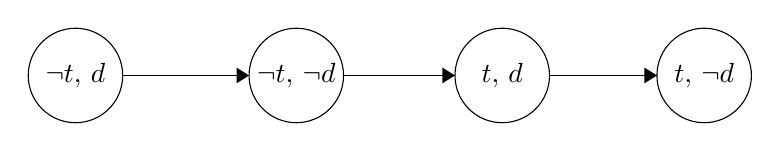
\begin{tikzpicture}[scale=0.2]
    \tikzstyle{every node}+=[inner sep=0pt]
    \draw [black] (51.233,-16.211) circle (3);
    \draw (51.23,-16.21) node {$t, \, d$};
    \draw [black] (24.133,-16.211) circle (3);
    \draw (24.13,-16.21) node {$\neg t, \, d$};
    \draw [black] (64.056,-16.211) circle (3);
    \draw (64.06,-16.21) node {$t, \, \neg d$};
    \draw [black] (38.156,-16.211) circle (3);
    \draw (38.156,-16.211) node {$\neg t, \, \neg d$};
    \draw [black] (54.23,-16.21) -- (61.06,-16.21);
    \fill [black] (61.06,-16.21) -- (60.26,-15.71) -- (60.26,-16.71);
    \draw [black] (27.13,-16.21) -- (35.16,-16.21);
    \fill [black] (35.16,-16.21) -- (34.36,-15.71) -- (34.36,-16.71);
    \draw [black] (41.16,-16.21) -- (48.23,-16.21);
    \fill [black] (48.23,-16.21) -- (47.43,-15.71) -- (47.43,-16.71);
    \end{tikzpicture}
    \end{center}

    \item \textit{Suppose somebody who never lies tells our agent ``You are
    close to the target if and only if you believe that you are in a dangerous
    zone.'' \textbf{Write down formally} this sentence as a formula $\varphi$
    in doxastic logic (using the atomic sentences).}

    $\varphi \coloneqq t \leftrightarrow B(d)$

    \item \textit{Interpreting the above truthful announcement $!\varphi$ as an
     \textbf{update} with the sentence $\varphi$ in the previous part,
    represent the \textbf{updated model}.}

    \begin{center}
    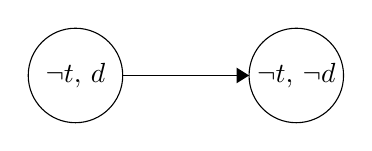
\begin{tikzpicture}[scale=0.2]
    \tikzstyle{every node}+=[inner sep=0pt]
    %\draw [black] (51.233,-16.211) circle (3);
    %\draw (51.23,-16.21) node {$t, \, d$};
    \draw [black] (24.133,-16.211) circle (3);
    \draw (24.13,-16.21) node {$\neg t, \, d$};
    %\draw [black] (64.056,-16.211) circle (3);
    %\draw (64.06,-16.21) node {$t, \, \neg d$};
    \draw [black] (38.156,-16.211) circle (3);
    \draw (38.156,-16.211) node {$\neg t, \, \neg d$};
    %\draw [black] (54.23,-16.21) -- (61.06,-16.21);
    %\fill [black] (61.06,-16.21) -- (60.26,-15.71) -- (60.26,-16.71);
    \draw [black] (27.13,-16.21) -- (35.16,-16.21);
    \fill [black] (35.16,-16.21) -- (34.36,-15.71) -- (34.36,-16.71);
    %\draw [black] (41.16,-16.21) -- (48.23,-16.21);
    %\fill [black] (48.23,-16.21) -- (47.43,-15.71) -- (47.43,-16.71);
    \end{tikzpicture}
    \end{center}

    \item \textit{After the previous announcement, another truthful
    announcement is made: ``You are in a dangerous zone if and only if you
    don't believe that you are in a dangerous zone.'' \textbf{Write down
    formally} this sentence as a formula $\psi$ in doxastic logic (using the
    atomic sentences).}

    $\psi \coloneqq d \leftrightarrow \neg B(d)$

    \item \textit{\textbf{What is the real world}? (In other words, answer the
    question: is the agent in a dangerous zone or not, and is he close to the
    target or not?) \textbf{Justify your answer}, by interpreting the
    announcement in the previous part as a new update $!\psi$ and
    \textbf{representing the updated model}.}

	Let S be the model of question 2.4. In S, $\psi$ holds only in world
	$(\neg t, \, d)$. In this world, $d$ is true and $\neg B(d)$ is true (because
	$B(d)$ is false, the agent believes $B(\neg d)$). In the other world,
	$(\neg t, \, \neg d)$, $d$ is false but $\neg B(d)$ is true, so $\psi$ doesn't
	 hold here. Because $\psi$ is truthful, the real world is $(\neg t, \, d)$.

    \begin{center}
    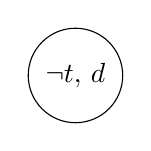
\begin{tikzpicture}[scale=0.2]
    \tikzstyle{every node}+=[inner sep=0pt]
    % \draw [black] (51.233,-16.211) circle (3);
    % \draw (51.23,-16.21) node {$t, \, d$};
    \draw [black] (24.133,-16.211) circle (3);
    \draw (24.13,-16.21) node {$\neg t, \, d$};
    % \draw [black] (64.056,-16.211) circle (3);
    % \draw (64.06,-16.21) node {$t, \, \neg d$};
    % \draw [black] (38.156,-16.211) circle (3);
    % \draw (38.156,-16.211) node {$\neg t, \, \neg d$};
    % \draw [black] (54.23,-16.21) -- (61.06,-16.21);
    % \fill [black] (61.06,-16.21) -- (60.26,-15.71) -- (60.26,-16.71);
    % \draw [black] (27.13,-16.21) -- (35.16,-16.21);
    % \fill [black] (35.16,-16.21) -- (34.36,-15.71) -- (34.36,-16.71);
    % \draw [black] (41.16,-16.21) -- (48.23,-16.21);
    % \fill [black] (48.23,-16.21) -- (47.43,-15.71) -- (47.43,-16.71);
    \end{tikzpicture}
    \end{center}

\end{enumerate}

\end{document}
